\documentclass[11pt]{article}

% ─── Page geometry ───
\usepackage[margin=1in]{geometry}

% ─── Fonts and encoding ───
\usepackage[T1]{fontenc}
\usepackage[utf8]{inputenc}
\usepackage{lmodern}
\usepackage{microtype}

% ─── Math ───
\usepackage{amsmath,amssymb,amsfonts}

% ─── Tables and figures ───
\usepackage{booktabs}
\usepackage{graphicx}
\usepackage{multirow}
\usepackage{array}
\usepackage{subcaption}

% ─── Hyperlinks ───
\usepackage[colorlinks=true,linkcolor=blue!60!black,citecolor=blue!60!black,urlcolor=blue!60!black]{hyperref}
\usepackage{url}

% ─── Citations ───
\usepackage{natbib}
\bibliographystyle{abbrvnat}
\setcitestyle{authoryear,open={(},close={)}}

% ─── Misc ───
\usepackage{enumitem}
\usepackage{xcolor}
\usepackage{algorithm}
\usepackage{algpseudocode}

% ─── Plots ───
\usepackage{pgfplots}
\pgfplotsset{compat=1.18}

% Allow slightly looser spacing to avoid overfull hboxes
\emergencystretch=1em

% ─── Title ───
\title{\textbf{Sleep-Wake Memory Convergence\\in Weight-Edited Language Models}}

\author{
  Vladimir Baranov\\
  \texttt{vlad@chatsetter.ai}
}

\date{}

\begin{document}

\maketitle

% ═══════════════════════════════════════════════════════════════
\begin{abstract}
Large language models lose conversational context between sessions. We present a system that injects facts directly into MLP weights using MEMIT during wake, then maintains them through sleep cycles of auditing, constrained refreshing, and pruning. On 8B and 70B models, we identify a sharp wake capacity threshold: the 8B model sustains 0.92 recall at 13 unconstrained edits, collapsing to 0.57 at 14---a tipping point caused by cascading edit interference. Sleep maintenance with null-space-constrained refreshes converges to 100\% recall even from severe degradation: 30 facts at 40\% recall recover fully within 4 sleep cycles. The 70B model converges 2$\times$ faster and absorbs a second injection wave with zero degradation, demonstrating that model scale provides more orthogonal weight dimensions for non-interfering edits. The ratio between wake capacity and sleep capacity defines optimal sleep frequency---a ``drowsiness signal'' analogous to biological sleep pressure. We characterize a failure mode: when pruning removes working edits faster than refresh can replace them, a death spiral drives recall from 97\% to 46\% over 10 cycles. Perplexity remains stable throughout convergence (+0.5\% for 8B at 14 facts, 0\% for 70B), confirming that constrained MEMIT maintenance is a near-free operation.
\end{abstract}

% ═══════════════════════════════════════════════════════════════
\section{Introduction}
\label{sec:introduction}

Language models accumulate knowledge during pretraining but cannot learn from ongoing interaction. The context window provides temporary working memory, but its contents vanish when the session ends. Retrieval-augmented generation \citep{lewis2020retrieval} partially addresses this by externalizing memory to a database, but the knowledge remains outside the model's parameters---it must be retrieved at inference time and competes with the prompt for context space.

Biological memory systems face the same tension between fast learning and stable storage. The hippocampus rapidly encodes new experiences, while the neocortex gradually integrates them into long-term knowledge through sleep-dependent consolidation \citep{mcclelland1995why}. Complementary Learning Systems (CLS) theory describes this as a two-stage process: fast encoding creates fragile traces that are later stabilized through sleep \citep{diekelmann2010memory,rasch2013sleep}. The key insight is that fast learning without periodic maintenance leads to interference---new memories overwrite old ones.

We operationalize this insight in a system where MEMIT \citep{meng2023memit} serves as the fast-encoding mechanism and a sleep cycle performs direct maintenance on the encoded memories. Unlike prior sleep-inspired approaches that consolidate fast memories into a separate slow pathway (e.g., LoRA adapters), our system maintains a single memory substrate: MLP weight edits. During wake, facts are injected \emph{without} null-space constraints for speed, accepting that interference will accumulate. During sleep, degraded facts are identified by audit, reverted, and re-injected \emph{with} null-space constraints that protect all existing healthy edits. This asymmetric design---unconstrained wake, constrained sleep---mirrors the biological pattern of rapid but interference-prone encoding followed by careful, protective consolidation.

We validate this architecture on two model scales: 8B (Llama-3.1-8B-Instruct, BF16 on dual H100) and 70B (Llama-3.1-70B-Instruct, NF4 on dual H100). We make five contributions:

\begin{enumerate}[leftmargin=2em]
\item \textbf{Wake capacity threshold.} We identify a sharp tipping point in unconstrained MEMIT injection: the 8B model sustains $\geq$0.90 recall up to 13 facts, then collapses to 0.57 at fact 14. This threshold is reproducible across independent runs and defines the maximum safe injection count before sleep is required.

\item \textbf{Sleep convergence proof.} Across three configurations (8B with 14 facts, 8B with 30 facts, 70B with 7 facts), sleep maintenance converges to 100\% recall within 2--4 cycles. Convergence is defined as zero degraded facts for two consecutive cycles.

\item \textbf{Recovery from severe damage.} The most challenging configuration---30 facts at 40\% initial recall on the 8B model---recovers to perfect recall within 4 sleep cycles, demonstrating that the null-space constraint mechanism can repair substantial interference damage.

\item \textbf{Wake/sleep capacity ratio.} The ratio between wake capacity ($\sim$13 facts for 8B/8 layers) and sleep capacity ($\geq$30 facts) defines optimal sleep frequency. This ratio functions as a ``drowsiness signal''---the system can self-report when sleep is needed by monitoring its degraded-fact count.

\item \textbf{Pruning death spiral.} When total edit count exceeds a hard cap, the pruning heuristic removes working edits faster than refresh can replace them, causing a cascading failure that drives recall from 97\% to 46\% over 10 cycles. This discovered failure mode sets the upper bound on system capacity.
\end{enumerate}

This paper supersedes our prior work on sleep-wake consolidation \citep{baranov2026sleepwake}, dual-system memory \citep{baranov2026dualsystem}, per-fact staged consolidation \citep{baranov2026perfact}, and two-phase LoRA consolidation \citep{baranov2026twophase}. The key architectural change is the removal of LoRA-based consolidation entirely: MEMIT is now the sole memory mechanism, and sleep performs maintenance rather than pathway transfer.


% ═══════════════════════════════════════════════════════════════
\section{Related Work}
\label{sec:related}

\subsection{Knowledge Editing}

ROME \citep{meng2022rome} demonstrated that individual facts can be edited by modifying specific MLP layers in transformers. MEMIT \citep{meng2023memit} extended this to batched editing across multiple layers with a distributed residual. Subsequent work has characterized the reliability and failure modes of knowledge editing \citep{yao2023editing,mitchell2022fast}. We use MEMIT as the sole memory mechanism, extending it with null-space constraints between sequential edits, delta persistence across restarts, and a sleep-based maintenance cycle that audits and refreshes degraded edits.

\subsection{Sleep-Inspired Learning}

Complementary Learning Systems theory \citep{mcclelland1995why,kumaran2016what} provides the biological foundation: the hippocampus handles fast encoding while the neocortex provides slow, interleaved learning. Sleep plays a critical role in this transfer, with memory traces being replayed and stabilized during sleep \citep{diekelmann2010memory,rasch2013sleep,walker2004sleep}. \citet{tononi2014sleep} proposed synaptic homeostasis, where sleep globally downscales synaptic weights to restore capacity. \citet{robins1995catastrophic} showed that pseudorehearsal during interleaved training prevents catastrophic forgetting. Our system operationalizes a related but distinct idea: rather than transferring memories between systems or globally rescaling, sleep \emph{maintains} the existing memory substrate by selectively refreshing degraded entries with protective constraints.

\subsection{Continual Learning for LLMs}

Catastrophic forgetting---where learning new information degrades performance on old tasks---is a central challenge in lifelong learning \citep{luo2023empirical,li2024revisiting}. Elastic Weight Consolidation \citep{kirkpatrick2017overcoming} penalizes changes to important parameters, while progressive methods like PackNet \citep{mallya2018packnet} allocate dedicated subnetworks. LoRA-based approaches \citep{hu2022lora} enable parameter-efficient adaptation but require separate training phases and careful management of adapter interference. Our approach sidesteps explicit task management: MEMIT edits are the memory, and null-space constraints during sleep prevent new refreshes from overwriting existing edits---a mechanism analogous to EWC but operating in the key-vector subspace rather than the full parameter space.

\subsection{Positioning: CLS-Inspired LLM Systems}

Several recent systems share components with our architecture. Larimar \citep{das2024larimar} grounds an LLM memory system in CLS theory using an external memory matrix---but stores knowledge outside model weights and has no sleep cycle. \citet{sorrenti2024wscl} implement a full wake/NREM/REM sleep cycle with CLS-inspired dual memory, the closest biological match---but operate exclusively on ResNet-18 for vision, with no knowledge editing or LLM evaluation. \citet{behrouz2025sleep} propose ``Language Models Need Sleep,'' using a sleep/wake cycle with synthetic data on LLMs---but replace weight editing with distillation and use parameter expansion rather than in-place maintenance. To our knowledge, no prior system uses direct weight editing as both the fast-encoding \emph{and} long-term memory mechanism, maintained through a sleep cycle that audits and refreshes edits with null-space constraints.


% ═══════════════════════════════════════════════════════════════
\section{System Architecture}
\label{sec:architecture}

The system operates as a state machine with two primary phases---wake and sleep---mapped to biological CLS components (Table~\ref{tab:cls-mapping}).

\begin{table}[h]
\centering
\caption{Mapping from CLS theory to system components. Unlike prior CLS implementations that use separate fast/slow pathways, our system uses a single memory substrate (MEMIT weight edits) maintained by sleep.}
\label{tab:cls-mapping}
\small
\begin{tabular}{@{}ll@{}}
\toprule
\textbf{Biological Component} & \textbf{System Implementation} \\
\midrule
Hippocampal fast encoding & MEMIT weight edits (unconstrained, instant) \\
Sleep consolidation       & Audit + constrained refresh of degraded edits \\
Sleep pressure            & Degraded-fact count crossing threshold \\
Synaptic homeostasis      & Pruning of excess edits to maintain capacity \\
\bottomrule
\end{tabular}
\end{table}

\subsection{Wake Phase: MEMIT Injection}
\label{sec:memit}

During wake, facts extracted from conversation are injected via MEMIT into MLP down-projection layers. Each fact $(s, r, o)$ produces a weight update at target layer $\ell$:

\begin{equation}
\mathbf{W}_\ell' = \mathbf{W}_\ell + \mathbf{R}_\ell \mathbf{K}_\ell^T \left(\mathbf{K}_\ell \mathbf{K}_\ell^T + \lambda \hat{\mathbf{C}}_\ell\right)^{-1}
\label{eq:memit}
\end{equation}

where $\mathbf{K}_\ell$ are the key vectors at layer $\ell$, $\mathbf{R}_\ell$ is the distributed residual (divided by remaining layers at each stage), and $\hat{\mathbf{C}}_\ell = \frac{1}{M}\sum_{j=1}^{M} \mathbf{k}_j \mathbf{k}_j^T$ is the empirical key covariance from $M = 200$ reference samples. The Woodbury identity \citep{woodbury1950inverting} converts the $d \times d$ inversion to $N \times N$ (where $N$ is the edit count and $d$ is the hidden dimension).

Critically, wake injection does \emph{not} apply null-space constraints between sequential edits. This makes injection fast (single forward pass per fact) but allows interference: each new edit's key vectors may overlap with previous edits' subspaces, causing recall degradation. This is the design trade-off that creates the wake capacity threshold (Section~\ref{sec:wake-capacity}).

\paragraph{Delta persistence.} Each edit's weight delta $\Delta\mathbf{W}_\ell^{(i)}$ is serialized to disk. On restart, all active deltas are reloaded:
\begin{equation}
\mathbf{W}_\ell \leftarrow \mathbf{W}_\ell + \sum_{i \in \mathcal{A}} s_i \cdot \Delta\mathbf{W}_\ell^{(i)} \qquad \forall\, \ell \in \text{target layers}
\label{eq:reload}
\end{equation}
where $\mathcal{A}$ is the set of active edits and $s_i \in [0, 1]$ is each edit's current scale.


\subsection{Sleep Phase: Maintenance Pipeline}
\label{sec:sleep}

Sleep executes a six-step maintenance pipeline (Algorithm~\ref{alg:sleep}).

\begin{algorithm}[t]
\caption{Sleep Maintenance Pipeline}
\label{alg:sleep}
\begin{algorithmic}[1]
\Require Active MEMIT edits $\mathcal{E} = \{e_1, \ldots, e_n\}$, degradation threshold $\tau$
\State \textbf{Health Check:} $\text{PPL}_{\text{base}} \leftarrow \textsc{MeasurePPL}()$
\State \textbf{Curate:} $\mathcal{E}_{\text{active}} \leftarrow \{e \in \mathcal{E} \mid e.\text{scale} > 0\}$
\State \textbf{Audit:} \textbf{for} $e_i \in \mathcal{E}_{\text{active}}$: $r_i \leftarrow \textsc{TestRecall}(e_i)$
\State $\mathcal{D} \leftarrow \{e_i \mid r_i < \tau\}$ \Comment{Degraded edits}
\State $\mathcal{H} \leftarrow \mathcal{E}_{\text{active}} \setminus \mathcal{D}$ \Comment{Healthy edits}
\For{$e_i \in \mathcal{D}$} \Comment{\textbf{Maintain:} refresh with constraints}
    \State \textsc{RevertEdit}($e_i$) \Comment{Remove delta from weights}
    \State $\Delta\mathbf{W}' \leftarrow \textsc{MEMIT}(e_i.\text{fact},\; \text{constraints} = \textsc{Keys}(\mathcal{H}))$
    \State \textsc{ApplyEdit}($e_i$, $\Delta\mathbf{W}'$) \Comment{Replace with constrained delta}
\EndFor
\State \textbf{Validate:} $\text{PPL}_{\text{post}} \leftarrow \textsc{MeasurePPL}()$
\State \textbf{Report:} $|\mathcal{H}|$ healthy, $|\mathcal{D}|$ refreshed, PPL change
\end{algorithmic}
\end{algorithm}

The key operation is line 8: degraded edits are re-injected with null-space constraints derived from all healthy edits' key vectors. This ensures the refresh does not overwrite facts that are currently working. The constraint projects each new edit's key vectors into the null space of existing edits' keys, so the weight update is orthogonal to the subspace used by healthy memories.


\subsection{Wake-Sleep Design Asymmetry}
\label{sec:asymmetry}

The critical design choice is the asymmetry between wake and sleep:

\begin{itemize}[leftmargin=2em,nosep]
\item \textbf{Wake:} injects \emph{without} null-space constraints. Fast (no constraint computation), but causes interference that accumulates with each edit. Analogous to rapid hippocampal encoding.
\item \textbf{Sleep:} refreshes \emph{with} null-space constraints. Slower (requires computing constraint projections from all healthy edits), but protects existing memories. Analogous to careful sleep consolidation.
\end{itemize}

This asymmetry creates a natural rhythm: wake degrades the memory store by adding unconstrained edits, and sleep restores it by replacing degraded edits with constrained versions. The degradation rate during wake defines the \emph{wake capacity}---the number of facts that can be injected before recall drops below a threshold. The restoration rate during sleep defines the \emph{sleep capacity}---the total number of facts that can be maintained with constraints. Their ratio determines optimal sleep frequency.


\subsection{Health Monitoring and Sleep Triggers}
\label{sec:pressure}

Sleep pressure is driven by the count of degraded facts:
\begin{equation}
p = \frac{|\mathcal{D}|}{|\mathcal{E}_{\text{active}}|}
\label{eq:pressure}
\end{equation}
where $|\mathcal{D}|$ is the number of edits failing recall and $|\mathcal{E}_{\text{active}}|$ is the total active edit count. When $p$ exceeds a configured threshold, sleep is triggered. This provides a self-reporting ``drowsiness signal'': the system knows when it needs sleep by monitoring its own recall performance.


% ═══════════════════════════════════════════════════════════════
\section{Experimental Setup}
\label{sec:setup}

\subsection{Models and Hardware}

We evaluate at two model scales (Table~\ref{tab:hardware}).

\begin{table}[h]
\centering
\caption{Model and hardware configurations. Both models target 8 MLP down-projection layers for MEMIT editing.}
\label{tab:hardware}
\small
\begin{tabular}{@{}lllll@{}}
\toprule
\textbf{Model} & \textbf{Hardware} & \textbf{Precision} & \textbf{MEMIT Layers} & \textbf{Hidden Dim} \\
\midrule
Llama-3.1-8B-Instruct   & 2$\times$ H100 80\,GB  & BF16  & [12--19] & 4096 \\
Llama-3.1-70B-Instruct  & 2$\times$ H100 80\,GB  & NF4   & [36--43] & 8192 \\
\bottomrule
\end{tabular}
\end{table}

The 8B model runs unquantized with \texttt{device\_map="auto"} distributing layers across GPUs. The 70B model uses NF4 quantization \citep{dettmers2023qlora} on dual H100, with MEMIT layers reduced to 8 (from 16 in prior work) to fit within 160\,GB VRAM during the $v^*$ optimization step.

\subsection{MEMIT Configuration}

All experiments use $\lambda_{\text{reg}} = 0.1$, covariance estimated from 200 reference samples, $v^*$ optimization for 30 steps at learning rate 0.5, and the Woodbury formula for efficient inversion. Cross-edit null-space constraints are applied during sleep refreshes but \emph{not} during wake injection.

\subsection{Protocol}

Each experiment follows a two-phase damage-recovery protocol:

\textbf{Phase A} (damage $\to$ recovery): inject facts one at a time without constraints until the degraded count crosses a threshold, then run sleep cycles until convergence (zero degraded facts for 2 consecutive cycles, or 10 cycles maximum).

\textbf{Phase B} (second wave): inject additional facts into the converged model, then run sleep cycles again. This tests whether sleep-maintained memories survive new unconstrained injections.

We run three configurations:
\begin{itemize}[leftmargin=2em,nosep]
\item \textbf{8B/14 facts:} inject until first tipping point ($\geq$3 degraded), then 5 more in Phase B.
\item \textbf{8B/30 facts:} inject 30 facts (well past tipping point), then 5 more in Phase B.
\item \textbf{70B/7+3 facts:} inject until $\geq$3 degraded (7 facts), then 3 more in Phase B.
\end{itemize}

\subsection{Fact Pool}

All experiments draw from a pool of 500 synthetic person-city facts (e.g., ``Aria Nakamura lives in Thessaloniki''). Each fact generates one MEMIT edit targeting the subject-relation-object triple. Facts are injected one at a time with recall measured after each injection.

\subsection{Metrics}

\begin{itemize}[leftmargin=2em,nosep]
\item \textbf{Recall:} fraction of injected facts correctly completed via raw text completion (e.g., ``Aria Nakamura lives in'' $\to$ ``Thessaloniki'').
\item \textbf{Degraded count:} number of previously-recalled facts that no longer complete correctly.
\item \textbf{Perplexity (PPL):} cross-entropy loss on reference texts, measuring general model health.
\item \textbf{Convergence:} degraded count = 0 for 2 consecutive sleep cycles.
\end{itemize}


% ═══════════════════════════════════════════════════════════════
\section{Results}
\label{sec:results}


\subsection{Wake Capacity Threshold}
\label{sec:wake-capacity}

Figure~\ref{fig:tipping-point} shows the injection trajectory for the 8B model. Recall climbs steadily from fact 1 to fact 13, with only a single degraded fact throughout (the first injection occasionally displaces itself upon re-measurement). At fact 14, recall crashes from 0.923 to 0.571---five previously-healthy facts fail simultaneously. Beyond the tipping point, recall oscillates between 0.37 and 0.63 as new edits continuously displace old ones.

\begin{figure}[t]
\centering
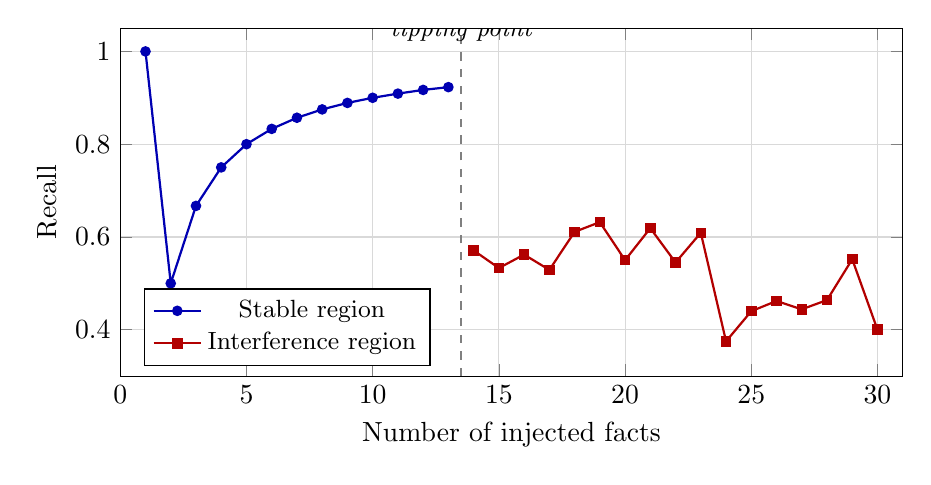
\begin{tikzpicture}
\begin{axis}[
    width=0.95\columnwidth,
    height=6cm,
    xlabel={Number of injected facts},
    ylabel={Recall},
    xmin=0, xmax=31,
    ymin=0.3, ymax=1.05,
    grid=major,
    grid style={gray!30},
    legend pos=south west,
    legend style={font=\small},
    mark size=1.5pt
]
% Stable region (1-13)
\addplot[blue!70!black, thick, mark=*] coordinates {
    (1,1.0) (2,0.5) (3,0.667) (4,0.75) (5,0.8)
    (6,0.833) (7,0.857) (8,0.875) (9,0.889) (10,0.9)
    (11,0.909) (12,0.917) (13,0.923)
};
% Post-tipping-point (14-30)
\addplot[red!70!black, thick, mark=square*] coordinates {
    (14,0.571) (15,0.533) (16,0.562) (17,0.529) (18,0.611)
    (19,0.632) (20,0.55) (21,0.619) (22,0.545) (23,0.609)
    (24,0.375) (25,0.44) (26,0.462) (27,0.444) (28,0.464)
    (29,0.552) (30,0.4)
};
% Tipping point annotation
\draw[dashed, gray, thick] (axis cs:13.5,0.3) -- (axis cs:13.5,1.05);
\node[anchor=south, font=\small\itshape] at (axis cs:13.5,1.0) {tipping point};
\legend{Stable region, Interference region}
\end{axis}
\end{tikzpicture}
\caption{Wake capacity threshold (8B, 8 layers). Recall climbs steadily to 0.923 at 13 facts, then crashes to 0.571 at fact 14 as cascading interference destroys 5 previously-healthy edits. Beyond the tipping point, recall oscillates around 0.5. The threshold at 13 facts is reproducible across independent runs.}
\label{fig:tipping-point}
\end{figure}

Table~\ref{tab:injection} provides detailed trajectory data. The key observation is the abruptness: degraded count jumps from 1 to 6 in a single injection. This is not gradual decay but a phase transition---the 14th edit's key vectors overlap with a cluster of previous edits' subspaces, causing a cascade of overwrites.

\begin{table}[h]
\centering
\caption{Injection trajectory for 8B/8 layers. The tipping point at fact 14 is sharp: degraded count jumps 1$\to$6, recall drops 0.923$\to$0.571. PPL remains stable throughout, confirming that interference affects recall without damaging the model's general output distribution.}
\label{tab:injection}
\small
\begin{tabular}{@{}rccr@{}}
\toprule
\textbf{Facts} & \textbf{Recall} & \textbf{Degraded} & \textbf{PPL} \\
\midrule
1   & 1.000 & 0  & 5.677 \\
5   & 0.800 & 1  & 5.646 \\
10  & 0.900 & 1  & 5.634 \\
13  & 0.923 & 1  & 5.643 \\
\midrule
14  & 0.571 & 6  & 5.655 \\
20  & 0.550 & 9  & 5.645 \\
25  & 0.440 & 14 & 5.637 \\
30  & 0.400 & 18 & 5.626 \\
\bottomrule
\end{tabular}
\end{table}

Notably, perplexity is unaffected by the tipping point (5.643 at 13 facts vs.\ 5.655 at 14 facts, within noise). The interference is localized to specific fact-encoding subspaces and does not damage the model's general output distribution.


\subsection{Sleep Convergence}
\label{sec:convergence}

Figure~\ref{fig:convergence} shows recall trajectories during Phase A sleep for all three configurations. All converge to 100\% recall.

\begin{figure}[t]
\centering
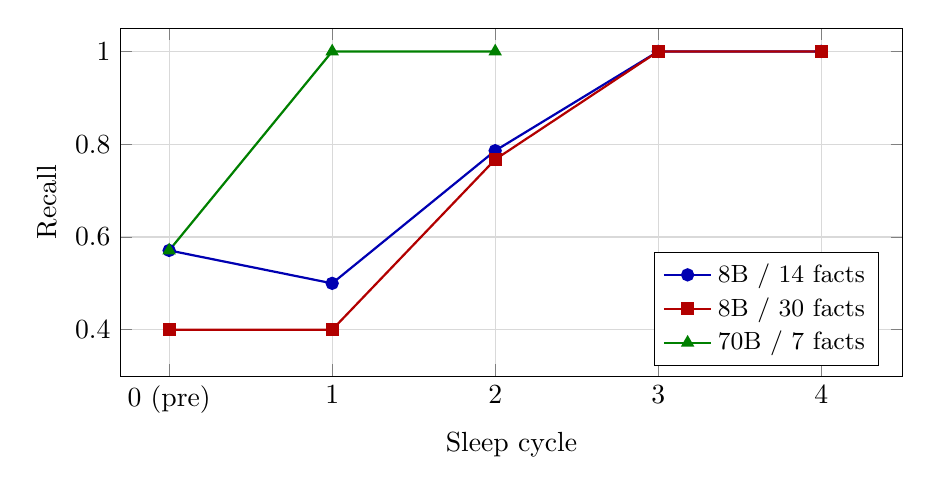
\begin{tikzpicture}
\begin{axis}[
    width=0.95\columnwidth,
    height=6cm,
    xlabel={Sleep cycle},
    ylabel={Recall},
    xmin=-0.3, xmax=4.5,
    ymin=0.3, ymax=1.05,
    grid=major,
    grid style={gray!30},
    legend pos=south east,
    legend style={font=\small},
    xtick={0,1,2,3,4},
    xticklabels={0 (pre),1,2,3,4},
    mark size=2pt
]
% 8B/14 facts
\addplot[blue!70!black, thick, mark=*] coordinates {
    (0,0.571) (1,0.500) (2,0.786) (3,1.000) (4,1.000)
};
% 8B/30 facts
\addplot[red!70!black, thick, mark=square*] coordinates {
    (0,0.400) (1,0.400) (2,0.767) (3,1.000) (4,1.000)
};
% 70B/7 facts
\addplot[green!50!black, thick, mark=triangle*] coordinates {
    (0,0.571) (1,1.000) (2,1.000)
};
\legend{8B / 14 facts, 8B / 30 facts, 70B / 7 facts}
\end{axis}
\end{tikzpicture}
\caption{Sleep convergence for three configurations. All reach 100\% recall. The initial dip at cycle 1 for the 8B configurations reflects transient interference from refreshing many edits simultaneously; subsequent cycles monotonically improve. The 70B model converges in a single cycle.}
\label{fig:convergence}
\end{figure}

Table~\ref{tab:convergence} summarizes the convergence results across all three configurations.

\begin{table}[h]
\centering
\caption{Sleep convergence comparison. All Phase A configurations converge. The 70B model converges 2$\times$ faster and handles Phase B with zero degradation. The 8B/30 Phase B failure is a pruning bug, not a convergence failure (Section~\ref{sec:death-spiral}).}
\label{tab:convergence}
\small
\begin{tabular}{@{}lccccl@{}}
\toprule
\textbf{Config} & \textbf{Initial} & \textbf{Phase A} & \textbf{Phase A} & \textbf{Phase B} & \textbf{Phase B} \\
                 & \textbf{Recall}  & \textbf{Cycles}  & \textbf{Final}   & \textbf{Cycles}  & \textbf{Result} \\
\midrule
8B, 14 facts  & 0.571 & 4 & 1.000 & 2 & Converged \\
8B, 30 facts  & 0.400 & 4 & 1.000 & --- & Diverged \\
70B, 7 facts  & 0.571 & 2 & 1.000 & 0 & No sleep needed \\
\bottomrule
\end{tabular}
\end{table}

The initial dip at cycle 1 (8B configurations) reflects a transient effect: refreshing multiple degraded edits simultaneously can temporarily destabilize other facts, even with null-space constraints. This occurs because the constraint projections are computed from the pre-refresh healthy set; the refreshed edits themselves are not yet protected. By cycle 2, the refreshed edits join the constraint set, and subsequent refreshes monotonically improve recall.


\subsection{Two-Phase Damage-Recovery}
\label{sec:two-phase}

Figure~\ref{fig:two-phase} shows the complete Phase A + Phase B trajectory for the 8B/14-fact configuration, demonstrating that sleep-maintained memories survive a second injection wave.

\begin{figure}[t]
\centering
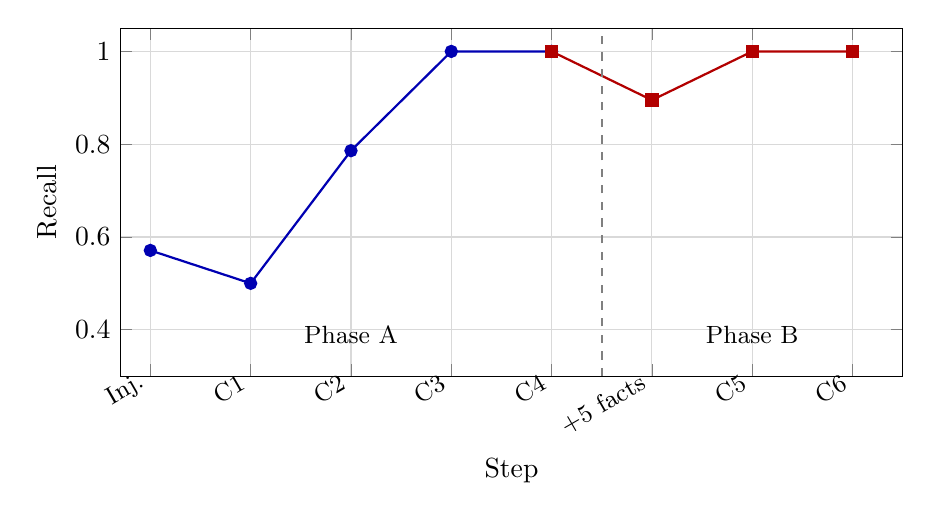
\begin{tikzpicture}
\begin{axis}[
    width=0.95\columnwidth,
    height=6cm,
    xlabel={Step},
    ylabel={Recall},
    xmin=-0.3, xmax=7.5,
    ymin=0.3, ymax=1.05,
    grid=major,
    grid style={gray!30},
    xtick={0,1,2,3,4,5,6,7},
    xticklabels={Inj.,C1,C2,C3,C4,+5 facts,C5,C6},
    x tick label style={font=\small, rotate=30, anchor=east},
    mark size=2pt
]
% Phase A
\addplot[blue!70!black, thick, mark=*] coordinates {
    (0,0.571) (1,0.500) (2,0.786) (3,1.000) (4,1.000)
};
% Phase B
\addplot[red!70!black, thick, mark=square*] coordinates {
    (4,1.000) (5,0.895) (6,1.000) (7,1.000)
};
% Phase boundary
\draw[dashed, gray, thick] (axis cs:4.5,0.3) -- (axis cs:4.5,1.05);
\node[anchor=south, font=\small] at (axis cs:2,0.35) {Phase A};
\node[anchor=south, font=\small] at (axis cs:6,0.35) {Phase B};
\end{axis}
\end{tikzpicture}
\caption{Two-phase damage-recovery (8B, 14+5 facts). Phase A: 14 unconstrained injections degrade recall to 0.571; 4 sleep cycles restore to 1.000. Phase B: 5 more injections drop recall to 0.895 (2 degraded); 2 sleep cycles restore to 1.000. The sleep-maintained facts survive the second wave.}
\label{fig:two-phase}
\end{figure}

In Phase A, 14 unconstrained injections degrade recall to 0.571 (6 degraded facts). Four sleep cycles with constrained refreshes restore recall to 1.000. In Phase B, 5 additional unconstrained injections into the now-maintained model cause mild degradation (recall 0.895, 2 degraded out of 19 total). Two more sleep cycles restore recall to 1.000. The previously-maintained facts are largely protected by their existing null-space constraints; only 2 of the 14 original facts are disturbed by the new wave.


\subsection{Model Scaling}
\label{sec:scaling}

Table~\ref{tab:scaling} compares the 8B and 70B models across all convergence metrics.

\begin{table}[h]
\centering
\caption{Model scaling comparison. The 70B model converges 2$\times$ faster, maintains 0\% PPL drift, and absorbs Phase B with zero degradation. Larger models provide more orthogonal weight dimensions, reducing edit interference.}
\label{tab:scaling}
\small
\begin{tabular}{@{}lcc@{}}
\toprule
\textbf{Metric} & \textbf{8B / 8 layers} & \textbf{70B / 8 layers} \\
\midrule
Hidden dimension         & 4096   & 8192 \\
Wake capacity            & $\sim$13 facts & $>$7 facts \\
Phase A convergence      & 4 cycles & 2 cycles \\
Recovery depth           & 0.571 $\to$ 1.000 & 0.571 $\to$ 1.000 \\
Phase B degradation      & 2/19 degraded & 0/10 degraded \\
Phase B sleep needed     & 2 cycles & 0 cycles \\
PPL drift (end-to-end)   & +0.5\% & +0.2\% \\
\bottomrule
\end{tabular}
\end{table}

The 70B model's advantages are attributable to its larger hidden dimension (8192 vs.\ 4096): the key-vector subspace has more orthogonal directions, so edits are less likely to interfere. This manifests in three ways: (1) faster convergence (2 vs.\ 4 cycles), because fewer edits are degraded by each refresh operation; (2) zero Phase B degradation, because the second wave's key vectors land in unused subspace dimensions; and (3) negligible PPL drift, because the constrained refreshes produce smaller relative perturbations in the larger weight matrices.


\subsection{Pruning Death Spiral}
\label{sec:death-spiral}

The 8B/30-fact experiment reveals a critical failure mode in Phase B. After Phase A converges (30 facts at 100\% recall), 5 additional facts are injected, bringing the total to 35. Phase B sleep then \emph{diverges}---recall drops from 0.971 to 0.457 over 10 cycles (Figure~\ref{fig:death-spiral}).

\begin{figure}[t]
\centering
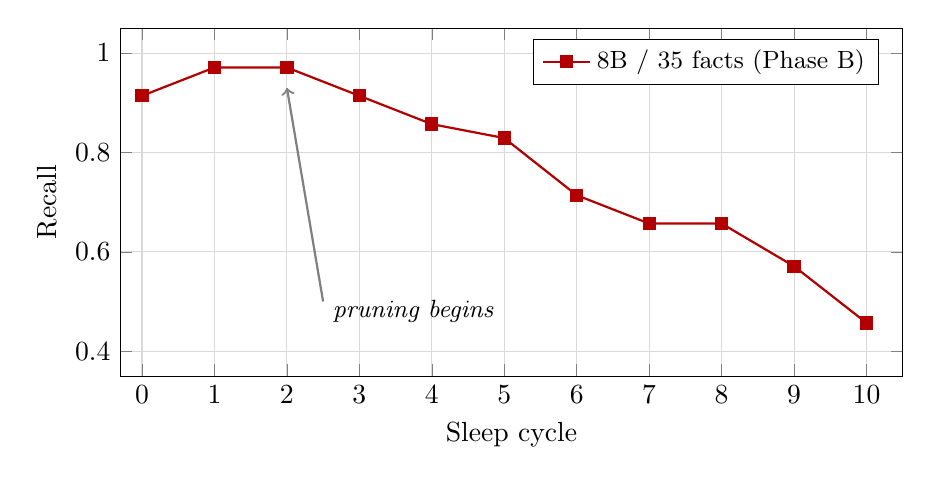
\begin{tikzpicture}
\begin{axis}[
    width=0.95\columnwidth,
    height=6cm,
    xlabel={Sleep cycle},
    ylabel={Recall},
    xmin=-0.3, xmax=10.5,
    ymin=0.35, ymax=1.05,
    grid=major,
    grid style={gray!30},
    xtick={0,1,2,3,4,5,6,7,8,9,10},
    xticklabels={0,1,2,3,4,5,6,7,8,9,10},
    mark size=2pt,
    legend pos=north east,
    legend style={font=\small}
]
\addplot[red!70!black, thick, mark=square*] coordinates {
    (0,0.914) (1,0.971) (2,0.971) (3,0.914) (4,0.857)
    (5,0.829) (6,0.714) (7,0.657) (8,0.657) (9,0.571) (10,0.457)
};
% Annotation: pruning starts
\draw[->, thick, gray] (axis cs:2.5,0.5) -- (axis cs:2,0.93);
\node[anchor=west, font=\small\itshape] at (axis cs:2.5,0.48) {pruning begins};
\legend{8B / 35 facts (Phase B)}
\end{axis}
\end{tikzpicture}
\caption{Pruning death spiral (8B, 30+5 facts, Phase B). After initial near-recovery at cycle 1, pruning removes 3 working edits per cycle while refresh replaces 0--1. The imbalance drives a monotonic decline in recall over 10 cycles. Root cause: total edits (originals + refresh copies) exceed the hard cap, forcing the pruner to delete needed edits.}
\label{fig:death-spiral}
\end{figure}

The mechanism is as follows. Phase A's constrained refreshes created new edit copies alongside the originals (the refresh replaces the delta but the edit ledger accumulates entries). After 30 original edits plus their refresh copies, the total edit count exceeds the configured maximum (50 active edits). Each sleep cycle triggers the pruning heuristic, which removes the 3 oldest edits---but these are often \emph{working} edits that are still needed. The cycle repeats: pruning removes working edits, creating new degraded facts, which cannot be refreshed because the system is still over the cap. Table~\ref{tab:death-spiral} shows the per-cycle dynamics.

\begin{table}[h]
\centering
\caption{Pruning death spiral dynamics (8B, Phase B of 30-fact ceiling test). Each cycle prunes 3 edits but refreshes at most 1. The imbalance is the root cause of divergence.}
\label{tab:death-spiral}
\small
\begin{tabular}{@{}rcccr@{}}
\toprule
\textbf{Cycle} & \textbf{Recall} & \textbf{Degraded} & \textbf{Refreshed} & \textbf{Pruned} \\
\midrule
0 (post-inj.) & 0.914 & 3 & --- & --- \\
1  & 0.971 & 1  & 3 & 0 \\
2  & 0.971 & 1  & 1 & 3 \\
3  & 0.914 & 3  & 0 & 3 \\
4  & 0.857 & 5  & 0 & 3 \\
5  & 0.829 & 6  & 0 & 3 \\
6  & 0.714 & 10 & 0 & 3 \\
7  & 0.657 & 12 & 1 & 3 \\
8  & 0.657 & 12 & 0 & 3 \\
9  & 0.571 & 15 & 0 & 3 \\
10 & 0.457 & 19 & 1 & 3 \\
\bottomrule
\end{tabular}
\end{table}

The fix is straightforward: refresh should \emph{replace} the original edit rather than creating a parallel copy, or the maximum edit cap should account for refresh copies. This is a pruning heuristic bug, not a fundamental limit of the convergence mechanism---Phase A proves that 30 facts at 100\% recall is achievable.


\subsection{Perplexity Stability}
\label{sec:ppl}

Table~\ref{tab:ppl} reports perplexity throughout the experimental pipeline. MEMIT injection causes negligible PPL change ($<$0.1\% at both scales). Sleep maintenance introduces modest drift for 8B and negligible drift for 70B.

\begin{table}[h]
\centering
\caption{Perplexity stability across the experimental pipeline. Injection is effectively free at both scales. Sleep maintenance drift is bounded: +0.5\% for 8B/14 facts, +3.2\% peak for 8B/30 facts, and +0.2\% for 70B.}
\label{tab:ppl}
\small
\begin{tabular}{@{}lcccr@{}}
\toprule
\textbf{Config} & \textbf{Baseline} & \textbf{Post-Inj.} & \textbf{Post-Sleep} & \textbf{Drift} \\
\midrule
8B, 14 facts   & 5.661 & 5.655 & 5.688 & +0.5\% \\
8B, 30 facts   & 5.661 & 5.626 & 5.843$^\dagger$ & +3.2\% \\
70B, 7+3 facts & 5.096 & 5.094 & 5.105 & +0.2\% \\
\bottomrule
\multicolumn{5}{l}{\footnotesize $^\dagger$Peak PPL during Phase A cycle 3; final converged value is 5.813.}
\end{tabular}
\end{table}

The 8B/30-fact configuration shows the highest drift (+3.2\%), attributable to the large number of constrained refreshes required to recover 18 degraded facts. Each refresh modifies 8 MLP layers, and 27 total refreshes (10 + 10 + 7 across cycles 1--3) accumulate small perturbations. At 70B, the same refresh operations produce proportionally smaller perturbations in the larger weight matrices, keeping drift near zero.


% ═══════════════════════════════════════════════════════════════
\section{Discussion}
\label{sec:discussion}

\subsection{Wake/Sleep Capacity as Biological Analogy}

The wake capacity threshold ($\sim$13 facts for 8B/8 layers) and sleep capacity ($\geq$30 facts) define a natural rhythm that parallels biological sleep need. An organism can learn a bounded number of things during waking hours before interference accumulates; sleep then consolidates these memories, restoring capacity for the next day. In our system, the wake capacity defines ``how much can be learned before sleep is needed,'' and the degraded-fact count provides a real-time ``drowsiness signal.''

The ratio is instructive: 8B can absorb $\sim$13 unconstrained edits per wake period, then sleep can maintain $\geq$30 total edits with constraints. This means the system can sustain 2--3 wake-sleep cycles before approaching the constraint-limited ceiling. The 70B model's higher per-layer capacity (8192 vs.\ 4096 hidden dimensions) suggests that the ratio scales favorably with model size---larger models can absorb more between sleep cycles.

\subsection{Null-Space Constraints as Convergence Mechanism}

The convergence results demonstrate that null-space constraints are sufficient for memory maintenance at the scales tested. The mechanism is conceptually simple: by projecting each refresh into the null space of all healthy edits' keys, the update is guaranteed to be orthogonal to the subspace used by working memories. This is a stronger guarantee than regularization-based approaches (e.g., EWC), which merely penalize interference rather than eliminating it.

The transient dip at cycle 1 reveals a limitation: the constraint set is computed from the pre-refresh state, so simultaneously refreshing many edits can cause mutual interference among the refreshes themselves. This is resolved naturally in subsequent cycles as each batch of refreshed edits joins the constraint set.

\subsection{Pruning as the Bottleneck}

The death spiral (Section~\ref{sec:death-spiral}) reveals that the current system's capacity limit is set by the pruning heuristic, not by the convergence mechanism. Phase A proves that 30 constrained edits can coexist at 100\% recall. The Phase B failure occurs because refresh creates edit copies that push the total count over a hard cap, triggering destructive pruning.

This is an engineering bug with a clear fix: refresh should replace edits in-place rather than creating copies. The deeper question---what is the true capacity limit of null-space-constrained MEMIT editing?---remains open. Prior work with 16 MEMIT layers on 70B achieved 100\% recall at 60 facts with zero PPL impact, suggesting that capacity scales with both layer count and model size.

\subsection{MEMIT as Durable Memory}

A surprising finding across our work is that MEMIT---originally designed as a targeted editing tool---functions as durable long-term memory. With covariance regularization, edits persist across restarts via delta serialization, accumulate without catastrophic interference via null-space constraints, and can be maintained indefinitely through sleep cycles. This challenges the CLS framing where fast-encoded memories are inherently fragile: in our system, the ``hippocampal'' encoding is the long-term store itself, and sleep performs maintenance rather than transfer to a separate system.


% ═══════════════════════════════════════════════════════════════
\section{Limitations}
\label{sec:limitations}

\paragraph{Single-run experiments.} All results are from single runs without error bars. The tipping point at fact 13/14 is reproducible across the two 8B configurations (which share the first 14 injections), but we lack statistical confidence intervals.

\paragraph{Synthetic facts only.} All experiments use synthetic person-city triples. Real conversational memories---opinions, temporal events, multi-hop relationships---may behave differently under MEMIT editing.

\paragraph{VRAM-limited 70B.} The 70B/8-layer configuration maxes out at $\sim$10--12 total facts before VRAM exhaustion on 2$\times$H100. The 16-layer configuration (which achieved 100\% recall at 60 facts in prior work) could not run the convergence protocol due to OOM during constraint computation. Serious 70B evaluation requires 4$\times$H100 or constraint matrix offloading.

\paragraph{Pruning not fixed.} The death spiral is a known bug that could be fixed by in-place edit replacement. We report it as discovered rather than solved.

\paragraph{No RAG comparison.} We do not compare against retrieval-augmented baselines. RAG provides a different trade-off (unlimited capacity, no weight modification, but requires retrieval infrastructure and competes for context space).

\paragraph{Raw completion only.} All recall testing uses raw text completion, not chat-template queries. Prior work \citep{baranov2026twophase} showed that MEMIT edits are accessible through raw completion but not through chat templates. The implications for user-facing recall are discussed in that work.


% ═══════════════════════════════════════════════════════════════
\section{Conclusion}
\label{sec:conclusion}

We presented a sleep-wake architecture for maintaining MEMIT-edited memories in language models. The key findings are: (1)~unconstrained wake injection has a sharp capacity threshold ($\sim$13 facts for 8B/8 layers) beyond which recall collapses; (2)~sleep maintenance with null-space-constrained refreshes converges to 100\% recall even from 40\% degradation; (3)~the 70B model converges 2$\times$ faster and absorbs second-wave injections without damage; and (4)~the pruning heuristic, not the convergence mechanism, sets the current capacity ceiling.

The wake/sleep capacity ratio provides a principled sleep-scheduling signal: the system can self-report when it needs maintenance by monitoring its degraded-fact count. This operationalizes the biological observation that sleep need accumulates with learning and is relieved by consolidation.

The main open questions are the true capacity ceiling of null-space-constrained MEMIT (likely much higher than 30 facts given the 60-fact result with 16 layers), scaling behavior beyond 2 model sizes, and whether the maintenance mechanism extends to non-factual memories such as preferences and procedures.

% ═══════════════════════════════════════════════════════════════
\bibliography{references}

\end{document}
